\setlength{\parindent}{10mm}
To \href{https://code.visualstudio.com/Download}{\textbf{\uline{Visual Studio Code}}} υποστηρίζεται και από \textbf{Windows},\textbf{Mac},\textbf{MacOs} και \textbf{Linux}.

\begin{enumerate}
    \item Κατεβάστε στον υπολογιστή σας το .ΝΕΤ της επιλογής σας \href{https://dotnet.microsoft.com/en-us/download/visual-studio-sdks}{\uline{εδώ}}.

    \item Ανοίξτε το .exe φάκελο που κατεβάσατε και ολοκληρώστε την εγκατάσταση του .ΝΕΤ. 

    \begin{figure*}[ht]
        \centering
        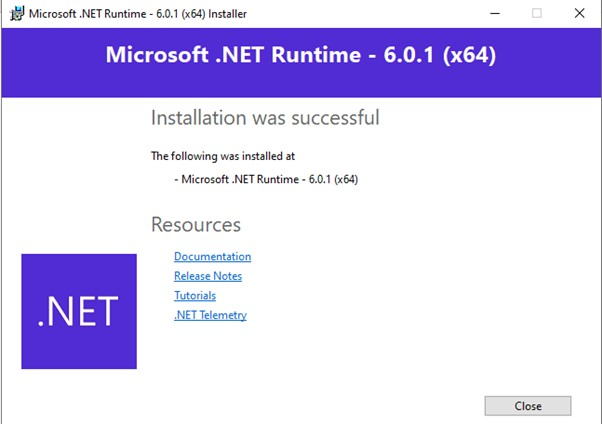
\includegraphics[scale=0.4]{images/instVSC1.jpg}
    \end{figure*}

    \item Ελέγξτε στο Command Channel αν η εγκατάσταση έγινε επιτυχώς πληκτρολογώντας \textbf{dotnet} - -\textbf{info}.

    \begin{figure*}[ht]
        \centering
        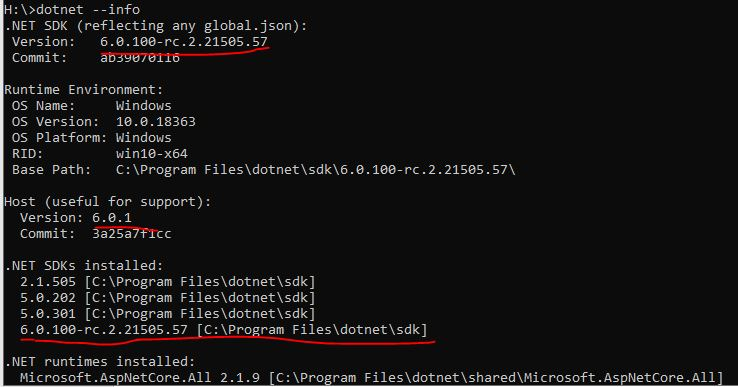
\includegraphics[scale=0.4]{images/instVSC2.jpeg}
    \end{figure*}

    Ελέγξτε ότι υπάρχουν τα αντίστοιχα υπογραμμισμένα στον υπολογιστή σας.
    \\[10\baselineskip]
    
    \item Κατεβάστε το VS Code ανάλογα με το λογισμικό του υπολογιστή σας \href{https://code.visualstudio.com/Download}{\uline{εδώ}}.

    \begin{figure*}[ht]
        \centering
        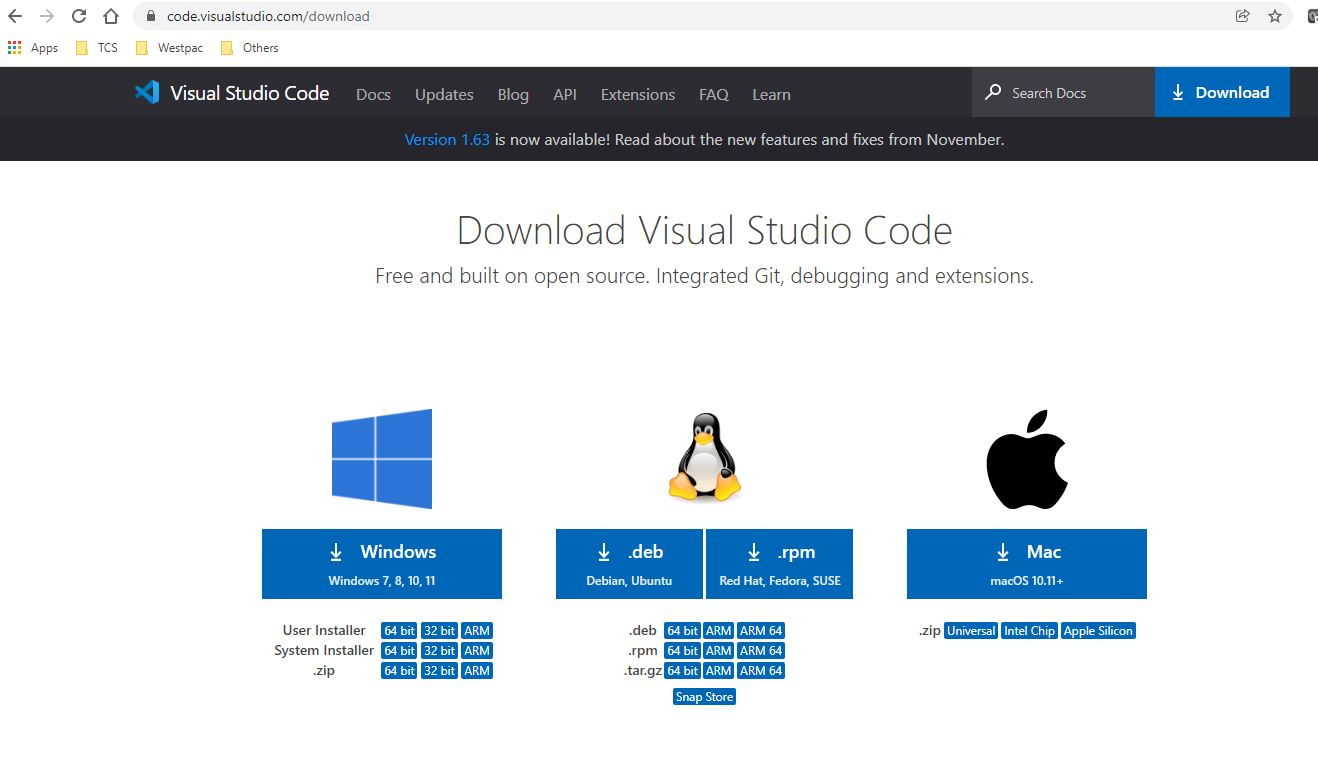
\includegraphics[scale=0.3]{images/instVSC3.jpeg}
    \end{figure*}

    \item Ανοίξτε τα Extensions του VS Code. \href{https://marketplace.visualstudio.com/VSCode}{\uline{εδώ}}

    Αναζητήστε και κατεβάσε την επέκταση για C\#. 

    \begin{figure*}[ht]
        \centering
        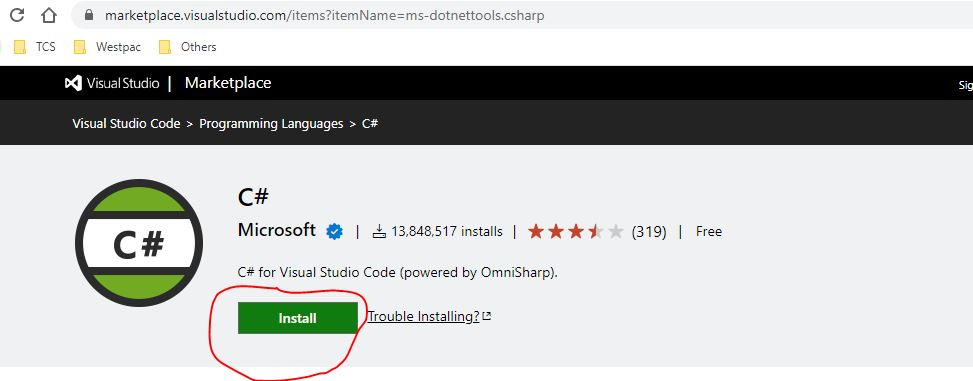
\includegraphics[scale=0.3]{images/instVSC4.jpeg}
    \end{figure*}

    Αυτό το βήμα μπορεί να γίνει και μέσα από το VS Code επιλέγοντας στο Menu Extension και αναζητώντας από εκεί την επέκταση για C\#.

    \item Ανοίξτε το VS Code στον υπολογιστή σας και δημιουργήστε εναν φάκελο Demo (ή μια ονομασία της επιλογής σας).Ανοίξτε αυτόν τον φάκελο ώστε να εμφαίζεται στα αριστερά του VS Code, στο μέρος που φαίνονται οι φάκελοι.
    \\[8\baselineskip]

    \item Ανοίξτε το terminal στο VS Code.
    \begin{figure*}[ht]
        \centering
        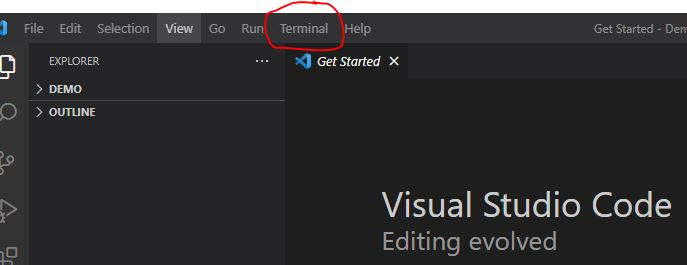
\includegraphics[scale=0.4]{images/instVSC5.jpeg}
    \end{figure*}

    \item Επιβεβαιώστε οτι βρίσκεστε στο σωστό Path αλλίως πλοηγηθείτε μέσω του terminal στο path που βρίσκεται το project (Demo) και πατήστε \textbf{dotnet new console}

    \begin{figure*}[ht]
        \centering
        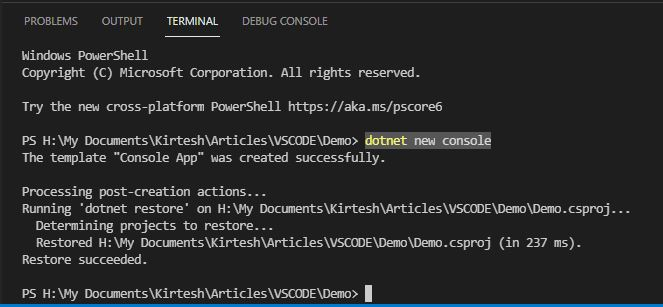
\includegraphics[scale=0.4]{images/instVSC6.jpeg}
    \end{figure*}

    \item Ελέγξτε ότι ο φάκελος Demo.csproj (εφόσον ονομάσατε το project Demo) περιλαμβάνει την έκδοση του .ΝΕΤ που εγκαταστήσατε όπως φαίνεται παρακάτω.

    \begin{figure*}[ht]
        \centering
        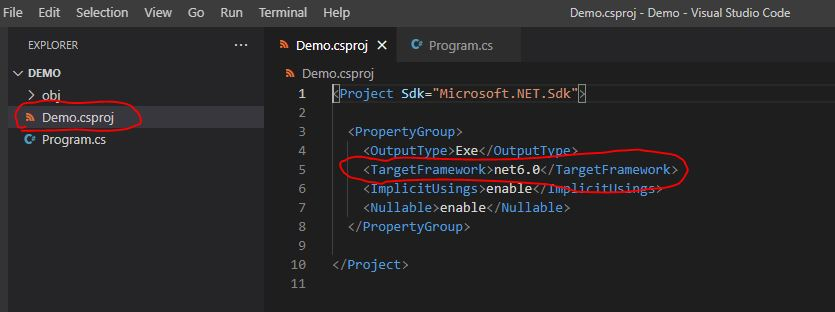
\includegraphics[scale=0.5]{images/instVSC7.jpeg}
    \end{figure*}

    Εφόσον όλα τα παραπάνω υλοποιήθηκαν σωστά. Γράψτε τον κωδικά σας στο program.cs.
    \\[8\baselineskip]

    \item Ο κώδικας σας θα εκτελεστεί πληκτρολογώντας στο terminal την εντολή \textbf{dotnet run}.

    \begin{figure*}[ht]
        \centering
        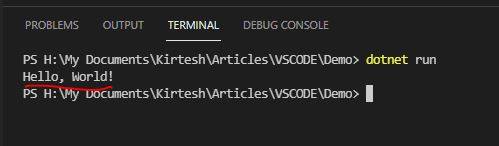
\includegraphics[scale=0.5]{images/instVSC8.jpeg}
    \end{figure*}
\end{enumerate}